\documentclass{article}

\usepackage[utf8]{inputenc}
\usepackage{float}
\usepackage{multirow}
\usepackage{hyperref}
\usepackage{todonotes}

\title{Mapping the Railway formalism onto different domains}
\author{Zhong Xi Lu}
\date{March 2019}

\begin{document}

\maketitle

\section{Introduction}

Modelling is a powerful technique which allows us to work on the right abstraction level and avoid accidental complexity. Nowadays, we have a lot of different formalisms at our disposal, so it's necessary to choose the most appropriate language when building a model. Aside from that, it's also possible to define a mapping from one formalism to another, so that we can expose the functionality of one another.

This paper will revolve around the \textit{Railway} formalism, which is mostly based on \textit{Railway Operation and Control} \cite{railway_book} by \textit{Joern Pachl} and some of the assignments \cite{assignments} given in the \textit{Model Driven Engineering} course in the \textit{University of Antwerp}. This formalism is first modelled in the tool \textit{AToMPM} \cite{atompm} to create a basic visual modelling environment, here we can also simulate a model by defining its operational semantics. To analyze if a model satisfies certain properties, we will map it to petri-nets, where we can do a reachability, coverability, deadlock, ... analysis. Next to that, we can also map it to \textit{Discrete Event System Specifications} (DEVS), which is more appropriate when it comes to queueing, throughput, ... analysis. Finally, to visualize and animate the model, we make use of \textit{Unity} \cite{unity}. \todo{finish introduction}

\todo{add diagram with the different formalisms}

\section{Railway Formalism}

As earlier mentioned, the book \textit{Railway Operation and Control} by \textit{Joern Pachl} \cite{railway_book} was a starting point for this Railway formalism. However, the language used in that book is heavily simplified to make the steps throughout this paper much easier. On top of that, the focus mainly lies on the railway (that consists of different segments) and not much on scheduling, signaling, ... This section will give a brief introduction on this simplified Railway formalism.

At its core, a model consists of multiple segments which can be connected to each other to form a railway. These segments also have a signalling light equipped which will inform an approaching train about its current state: green light means that there's no train represent on the segment and red light means there is. The different types of segments supported by this formalism can be found in table \ref{types_segments}.

\begin{table}[H]
\begin{tabular}{|l|l|l|}
\hline
\textbf{Name:}                 & \textbf{Symbol:} & \textbf{Description:}                                                                                                                                                                      \\ \hline
Straight                       & 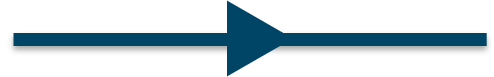
\includegraphics[scale=0.25]{images/straight} & \begin{tabular}[c]{@{}l@{}}a basic segment that connects and is connected\\ by one other segment\end{tabular}                                                                              \\ \hline
Start                          & 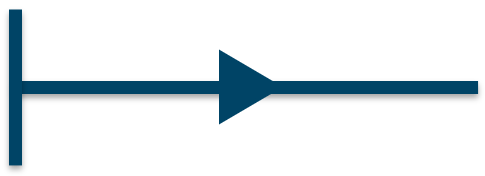
\includegraphics[scale=0.25]{images/start} & a segment with only an outgoing rail                                                                                                                                                       \\ \hline
End                            & 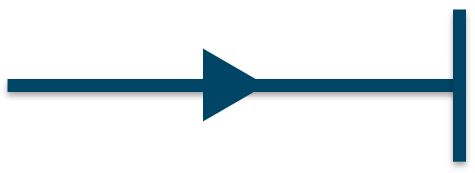
\includegraphics[scale=0.25]{images/end} & a segment with only an incoming rail                                                                                                                                                       \\ \hline
Turnout                        & 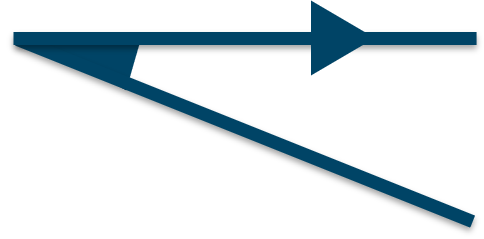
\includegraphics[scale=0.25]{images/turnout1} & \begin{tabular}[c]{@{}l@{}}a segment with internally a switch, which can be\\ used to control its outgoing rail (either going \\ straight or make a turn)\end{tabular}                     \\ \hline
Junction                       & 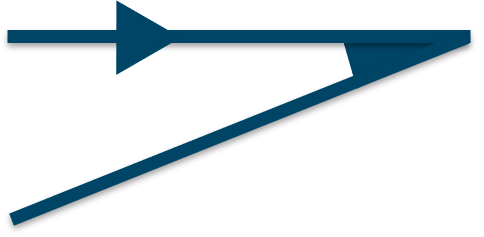
\includegraphics[scale=0.25]{images/junction1} & \begin{tabular}[c]{@{}l@{}}similar to a turnout, but instead of controlling its\\ outgoing rail, it will control the ingoing rail\\ (trains can arrive straight or in a turn)\end{tabular} \\ \hline
Crossing                       & 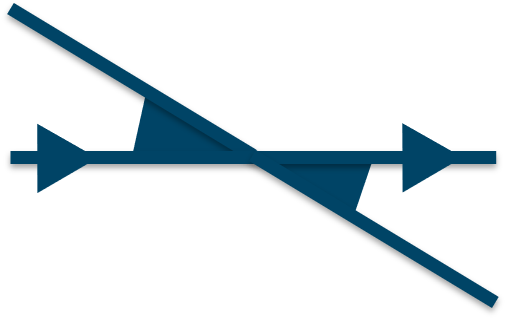
\includegraphics[scale=0.25]{images/crossing21} & \begin{tabular}[c]{@{}l@{}}a combination of a turnout and a junction, has two\\ switches available, allowing to control both the\\ incoming and outgoing rails\end{tabular}                \\ \hline
Station                        & 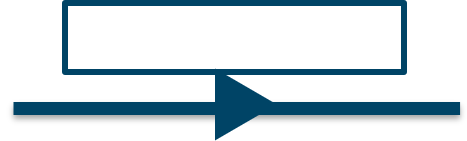
\includegraphics[scale=0.25]{images/station} & a segments with a train station next to it                                                                                                                                                 \\ \hline
\end{tabular}
\caption{All the different types of segments supported by the Railway formalism}
\label{types_segments}
\end{table}

\section{Abstract and Concrete Syntax}

Now that we have defined the initial concepts of our formalism, we can start by building the syntax. This is split in two parts, namely the abstract and concrete syntax. For more information on this topic, I refer to \textit{AToMPM}'s documentation \cite{atompm_docs}.

\subsection{Abstract Syntax}

\begin{figure}[H]
    \begin{center}
        \makebox[\textwidth]{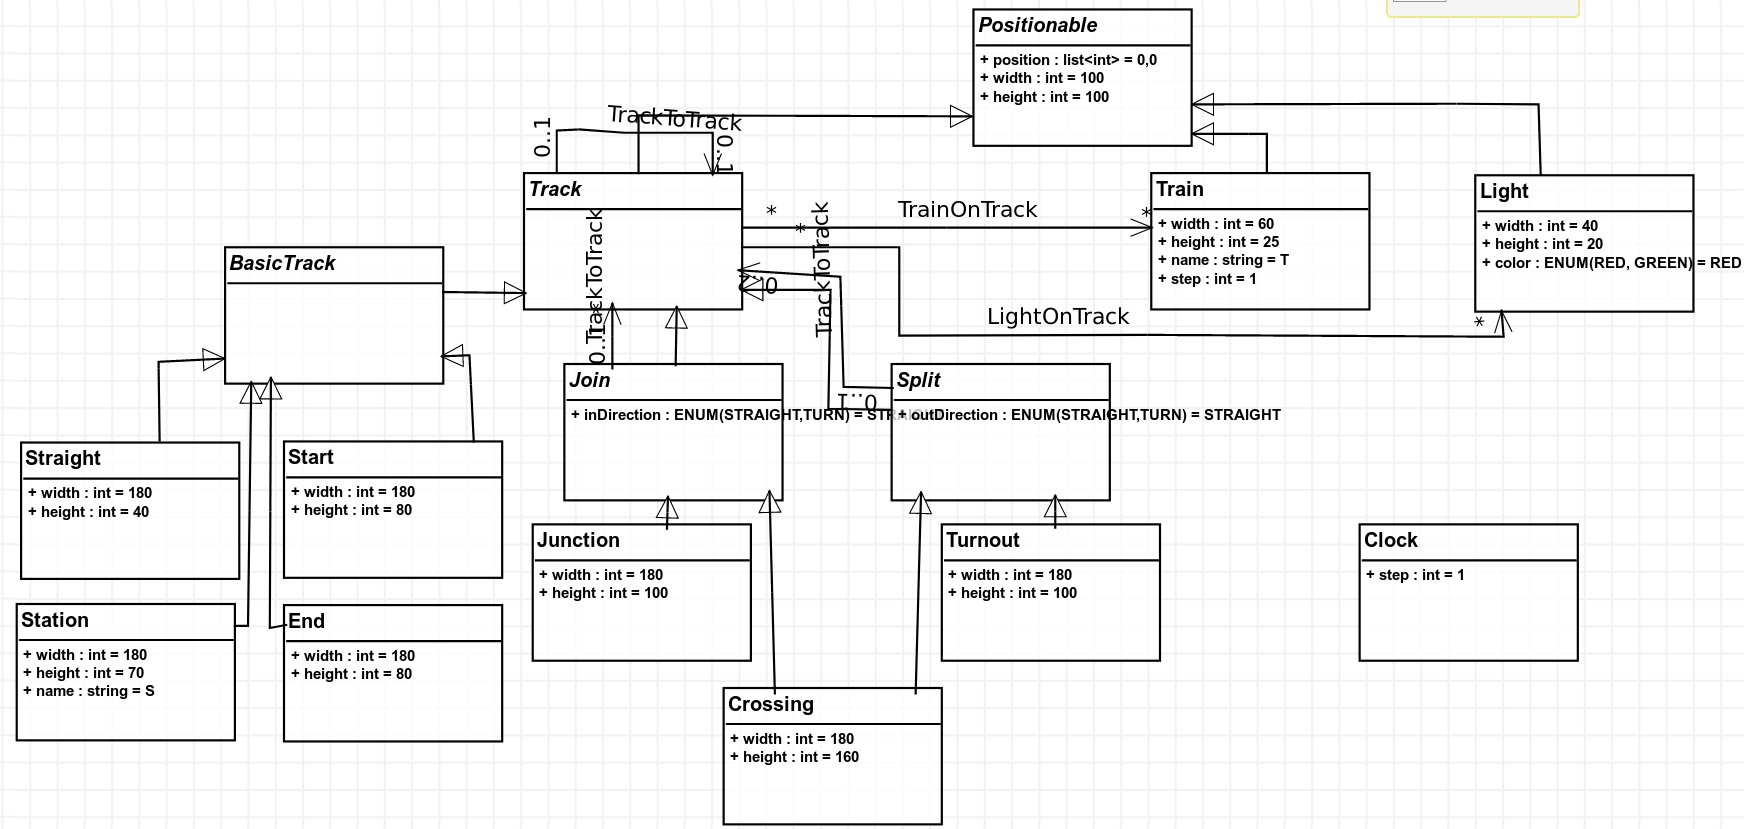
\includegraphics[width=0.9\paperwidth]{images/abstract_syntax}}
    \end{center}
    \caption{Abstract syntax of the Railway formalism}
    \label{abstract_syntax}
\end{figure}

Since we deal with multiple types of segments, an inheritance tree would be suitable for this problem. At the root, we have an abstract class \texttt{Track}, from here on, we have three (abstract) subclasses:

\begin{itemize}
    \item \texttt{BasicTrack}: All the most basic tracks that have at most one incoming and outgoing track (\texttt{Start} does not have an incoming track and \texttt{End} not an outgoing one).
    \item \texttt{Join}: A track where two incoming tracks converge, in other words, a junction. It also has an attribute (\texttt{inDirection}) which tells in which the switch is set.
    \item \texttt{Split}: A track that has two outgoing tracks. Similar to \texttt{Join}, this also has an attribute (\texttt{outDirection}) to indicate the current direction of the outgoing track.
\end{itemize}

To actually connect the tracks to one another, the \texttt{TrackToTrack} link is used, by default a \texttt{Track} can only connect and be connected by one other track. However, there are of course segments where this is not the case and where we have to override the existing cardinality constraint constraint; for example, \texttt{Join}s can have two incoming one's and \texttt{Split}s two outgoing one's. This link also has an extra attribute \texttt{direction} to store to which "port" it has been connected in case it's connected to a junction; for example \texttt{STRAIGHT} means that it is connected to the \texttt{STRAIGHT} rail of the junction.

Aside from track, we can also create \texttt{Train}s, which is self-explanatory, and \texttt{Light}s that are used for signalling purposes. These objects can of course be linked and placed on tracks, this is managed by the \texttt{TrainOnTrack} and \texttt{LightOnTrack} links. Finally, a \texttt{Clock} is explicitly modelled here as well, this is to keep track of the simulation steps and make the simulation process easier later on.

Note that there are some "visual" attributes present in the model: \texttt{position}, \texttt{width} and \texttt{height}. These attributes are mainly used to automatically connect segments to each other when they are linked. In true nature, this is not the ideal method to store this in the abstract syntax, but this is just a slight work around to store some visual information. As such, there exists an abstract base class \texttt{Positionable} to deal with this.

\subsection{Concrete Syntax}

\begin{figure}[H]
    \begin{center}
        \makebox[\textwidth]{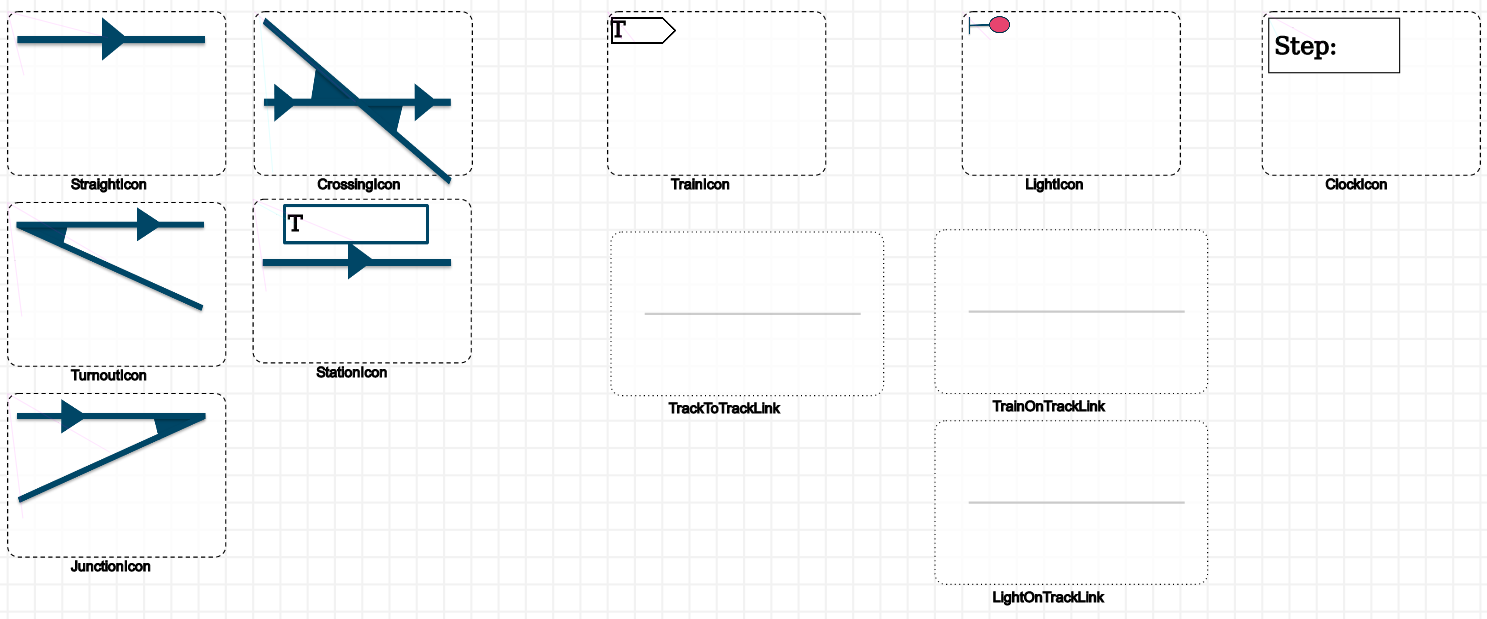
\includegraphics[width=0.8\paperwidth]{images/concrete_syntax.png}}
    \end{center}
    \caption{Concrete syntax of the Railway formalism}
    \label{concrete_syntax}
\end{figure}

Having modelled the abstract syntax, we can now define the icons for our formalism (see figure \ref{concrete_syntax}). Most of these notation are based on the one used in the book \textit{Railway Operation and Control} by \textit{Joern Pachl} \cite{railway_book}. Besides that, these icons also change depending on the state; for example, a junction will show the current direction of the switch (indicated by the arrow). Either way, most these symbols are pretty straightforward.

\section{Operational Semantics}

This section will go over the operation semantics of the Railway formalism, i.e. how the whole system behaves and operates. To model this, we make use of transformation rules, again I refer to \textit{AToMPM}'s documentation \cite{atompm_docs} for more detail.

\subsection{Train Schedule Formalism}

Before we implement the rules, a second domain specific language is modelled to define train schedules (the path it takes from start to end) as was suggested in the \cite{assignments} given in the \textit{Model Driven Engineering} course \cite{assignments}. This way, we can easily operate the switches by looking at the train schedules.

The abstract syntax can be found in figure \ref{abstract_syntax_trainschedule} and the concrete in figure \ref{concrete_syntax_trainschedule}. Basically, a schedule consists of one startion station and one ending station. In between are zero or more steps that tell in which direction the train should move when it encounters a waypoint (turnout or crossing). One schedule is associated with  exactly one train and vice versa.

\begin{figure}[H]
    \centering
    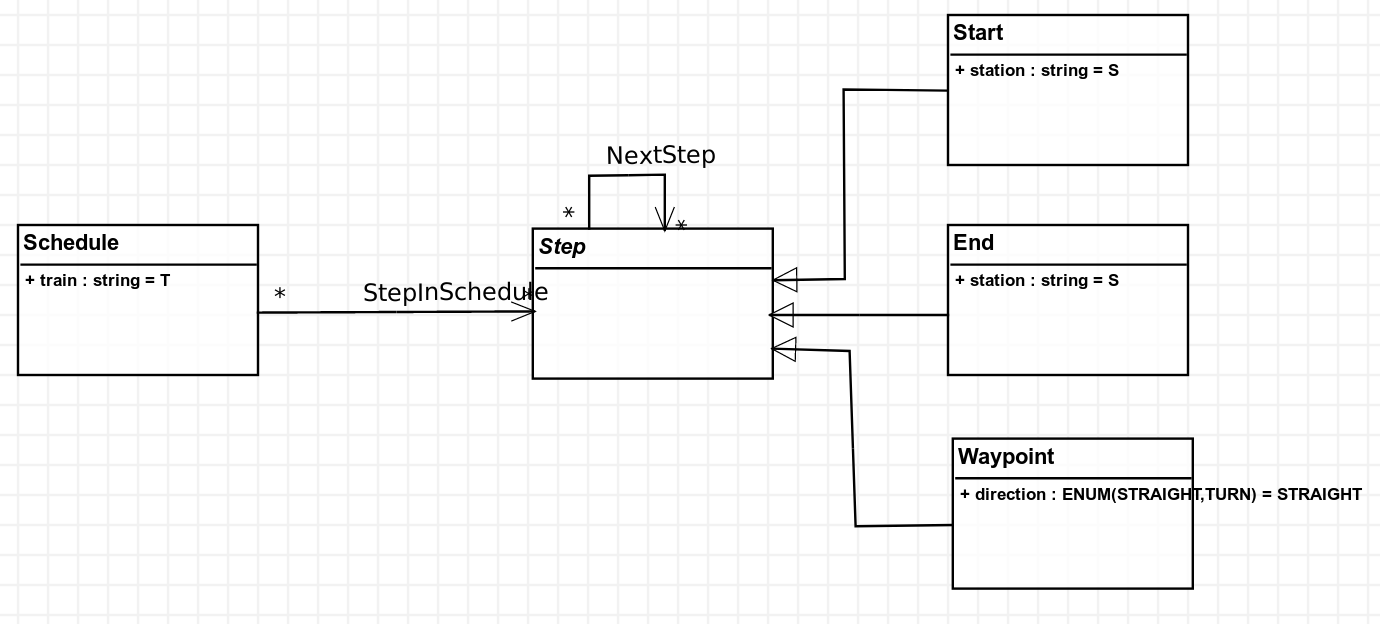
\includegraphics[width=\textwidth]{images/trainschedule_abstract_syntax.png}
    \caption{Abstract syntax of the Train Schedule formalism}
    \label{abstract_syntax_trainschedule}
\end{figure}

\begin{figure}[H]
    \centering
    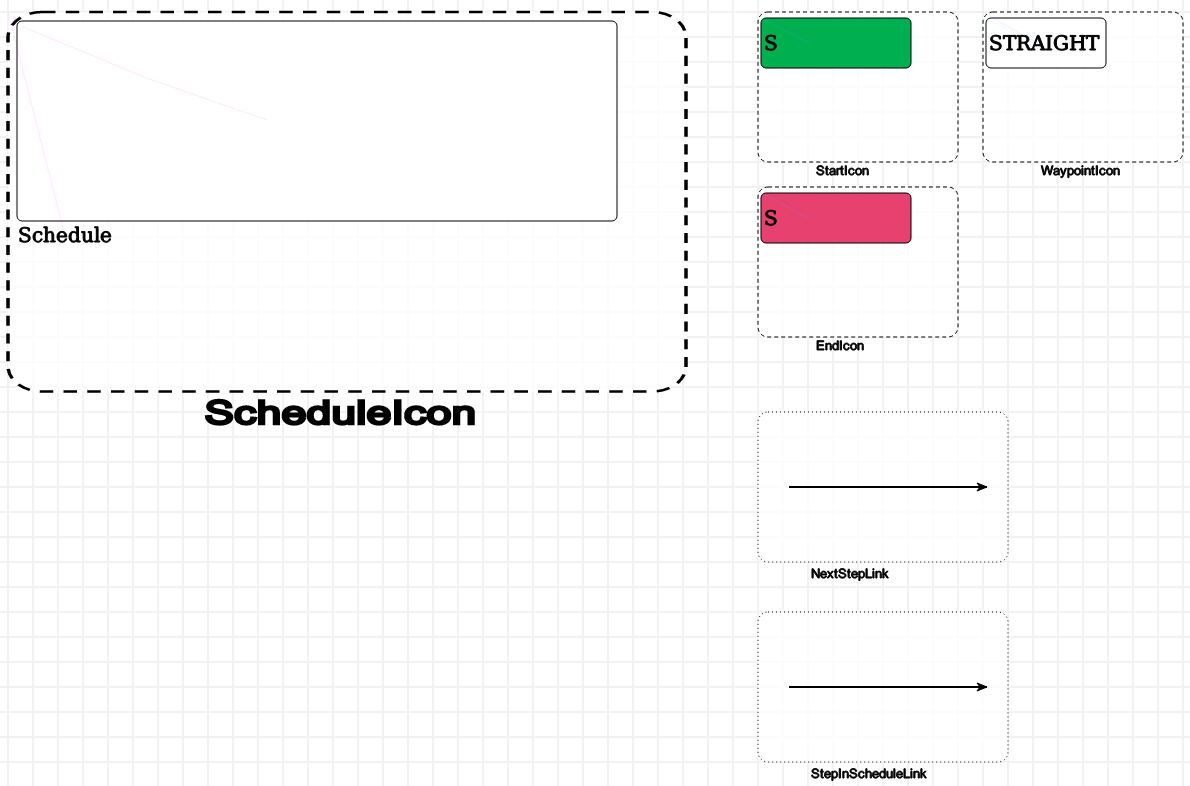
\includegraphics[width=\textwidth]{images/trainschedule_concrete_syntax.png}
    \caption{Concrete syntax of the Train Schedule formalism}
    \label{concrete_syntax_trainschedule}
\end{figure}

\subsection{Operational Semantics}

\begin{figure}[H]
    \centering
    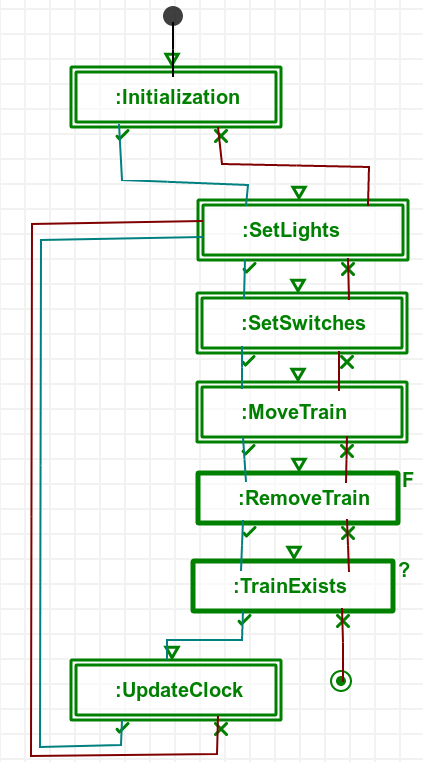
\includegraphics[width=0.4\textwidth]{images/schedule_opsem.png}
    \caption{Schedule for the operational semantics}
    \label{schedule_opsem}
\end{figure}

To explain the semantics, I will go over the MoTif schedule (figure \ref{schedule_opsem}):

\begin{enumerate}
    \item Initialization: Adds signalling lights to all tracks if that wasn't the case already and it will place all the trains on their starting station according to their unique train schedule.
    \item Set Lights: Set the lights correctly depending on their state; set the light green if there's no train present and red otherwise.
    \item Set switches: Set the switches on splits and joins:
        \begin{itemize}
            \item Joins: if a train wants to enter a junction, the control system will set the direction of the incoming track correctly so that the train can enter. If two trains want to enter, it will "randomly" choose one.
            \item Split: to set the switch for splits, we look at the train schedule of the train that is currently on this split. This schedule will tell us in which direction we should move. (see figure \ref{set_split_switch})
            \begin{figure}[H]
                \centering
                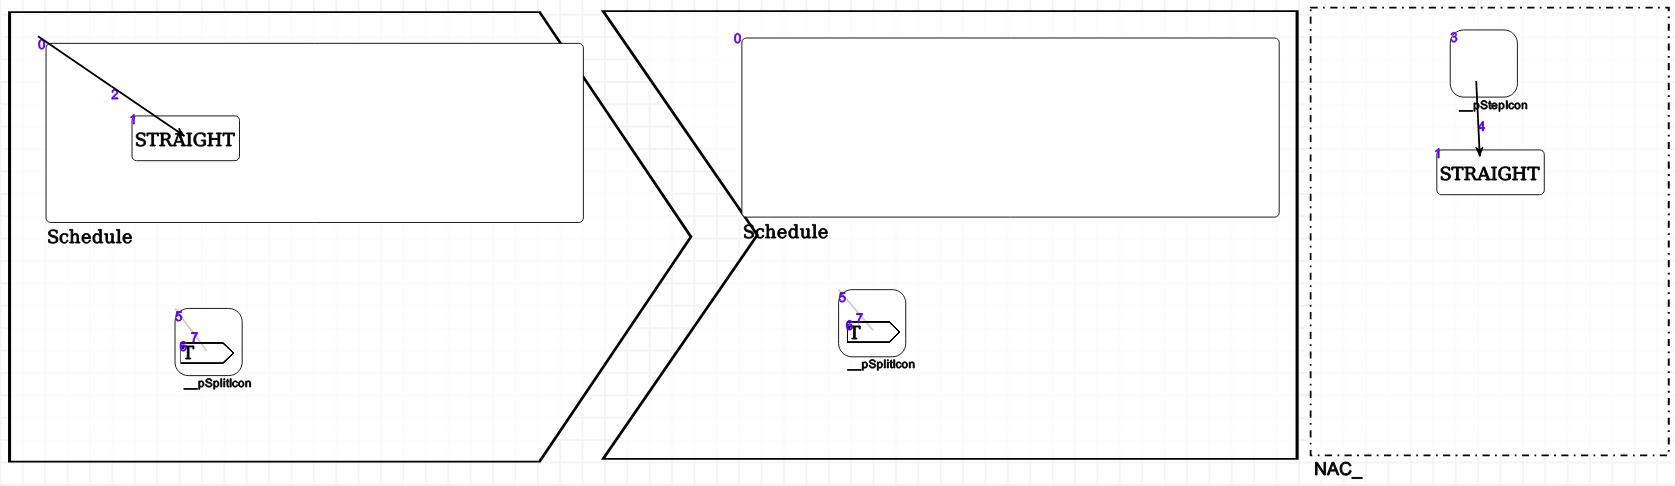
\includegraphics[width=\textwidth]{images/SetSplitSwitch.png}
                \caption{Transformation rule for setting switch on splits}
                \label{set_split_switch}
            \end{figure}
        \end{itemize}
    \item Move Train: This step will try to move a train to the next segment. There are however several cases that we have to keep in mind; for example, we can only move if the light on the next section is green. Most of these cases verify if the in/out-direction is set correctly.
    \item Remove Train: Whenever a train reaches its end (station), we will remove it from the model, so that potential future train can enter this station as well.
    \item Train Exists: A simple query rule to check if there are still trains left on any track. This is the end condition and the transformation will halt if there cannot be a train found.
    \item Update Clock: Finally, if the \texttt{TrainExists} was successful, we can move to the next simulation cycle: this step will update the clock as well as the step internally of all the trains so that they are synchronized with the clock.
\end{enumerate}

\section{Mapping to Petri-Nets}

\section{Mapping to DEVS}

\section{Conclusion}

\bibliographystyle{ieeetr}
\nocite{*}
\bibliography{references}

\end{document}
